\section{Data Cleaning and Preprocessing}
\noindent
Before analyzing this dataset, it must be cleaned and processed in order to derive accurate insights and predictive models.

\subsection{Reporting Sources}
\noindent
The data was compiled from two sources, Bing and MapQuest. These sources report severity differently, thus I had to decide which source to utilize. 

\begin{figure}[H]
    \centering
    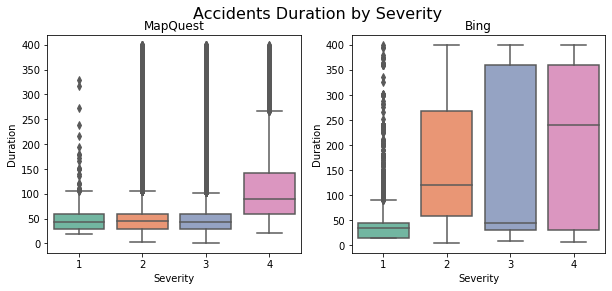
\includegraphics[width=115mm,height=\textheight,keepaspectratio]{images/duration_severity.png}
    \caption{Accident Duration by Severity}
    \label{fig:duration_severity}
\end{figure}

\begin{figure}[H]
    \centering
    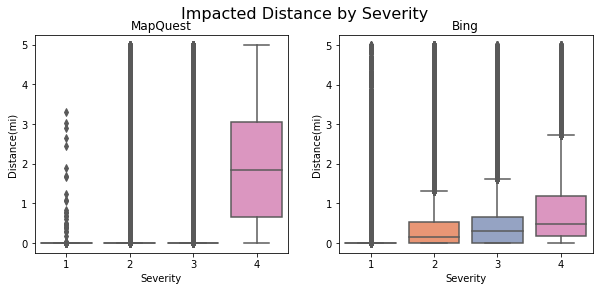
\includegraphics[width=115mm,height=\textheight,keepaspectratio]{images/distance_severity.png}
    \caption{Impacted Distance by Severity}
    \label{fig:distance_severity}
\end{figure}

As can be seen by \cref{fig:duration_severity,fig:distance_severity}, MapQuest has a clearly higher quartile 1, quartile 2 (median), and quartile 3 for severity 4. Bing seems to have a looser definition as the box and whisker plots are not too statistically significant from each other. For these reasons, I decided to only utilize the MapQuest data.

\subsection{Non-Predictive Features}
Data for columns 'ID', 'Distance(mi)', 'End Time', 'Duration', 'End Latitude', and 'End Longitude' can only be collected after the accident has already happened and hence cannot be used to predict severe accidents. Furthermore, since categorical variables like 'Country' and 'Turning Loop' only have one class, they cannot be predictive features as the probabilistic surprise and entropy for these random variables is 0 \citep{lesne2014shannon}.

\subsection{Filtering Incomplete Data}
Though this dataset is mostly complete, some entries lack data for certain columns. Rather than removing these columns for all entries, I decided to remove the incomplete row entries instead as the original dataset contains over 7.7 million accidents. Even after this filtering, there is still ample data.

